\documentclass[a4paper,12pt]{article}

\usepackage{mystyle}
\usepackage{gensymb}

\usepackage{scalerel}
\usepackage{stackengine}

\graphicspath{ {images/} }


\definecolor{violet}{RGB}{148, 0, 211}
\definecolor{pink}{RGB}{218, 3, 174}


% https://tex.stackexchange.com/a/101138/135045

\newcommand\widesim[1]{\ThisStyle{%
  \setbox0=\hbox{$\SavedStyle#1$}%
  \stackengine{-.1\LMpt}{$\SavedStyle#1$}{%
    \stretchto{\scaleto{\SavedStyle\mkern.2mu\sim}{.5150\wd0}}{.6\ht0}%
  }{O}{c}{F}{T}{S}%
}}

\newcommand{\BigMiddleThree}{\;\left|\vphantom{\begin{pmatrix} 0\\0\\0 \end{pmatrix}}\right.\;}
\newcommand{\BigMiddleFour}{\;\left|\vphantom{\begin{pmatrix} 0\\0\\0\\0 \end{pmatrix}}\right.\;}


\author{Алексеев Василий}


\title{Семинар 4}
\date{28 февраля + 3 марта 2023}


\begin{document}
  \maketitle
  
  \tableofcontents

  \thispagestyle{empty}
  
  \newpage
  
  \pagenumbering{arabic}


  \section{Линейные пространства 2}
  
  \subsection{Пересечение, сумма, прямая сумма, или ``Объединение: Они не знают, что ``подпространство''~---~это объединение слов ``под'' и ``пространство''}
  
  Приведём сразу определения понятий, которым посвящён конспект.
  
  \begin{definition}
    \emph{Пересечением} двух подпространств $L_1$ и $L_2$ линейного пространства $L$ называется подпространство, вектора которого~---~пересечение множеств векторов подпространств $L_1$ и $L_2$:
    \[
      L_1 \cap L_2 = \{\bds v \mid \bds v \in L_1, \bds v \in L_2\}
    \]
  \end{definition}
  
  Не сложно убедиться в том, что пересечение подпространств~---~это в самом деле тоже подпространство:
  \[
    \bds x, \bds y \in L_1 \cap L_2 \Rightarrow \bds x + \bds y \in L_1 \cap L_2
  \]
  \[
    \bds x \in L_1 \cap L_2, \alpha \in \RR \Rightarrow \alpha \bds x \in L_1 \cap L_2
  \]
  
  \begin{definition}[Сумма]
    \emph{Суммой} двух подпространств $L_1$ и $L_2$ линейного пространства $L$ называется линейная оболочка объединения векторов подпространств $L_1$ и $L_2$:
    \[
      L_1 + L_2 = \mathcal L(L_1 \cup L_2)
    \]
  \end{definition}
  
  Сумма подпространств~---~тоже подпространство.
  Потому что если $\bds x$ и $\bds y$ находятся в $L_1 \hm+ L_2$, то они каждый являются линейными комбинациями векторов $L_1 \hm\cup L_2$.
  Очевидно, что и сумма $\bds x \hm+ \bds y$, и результат умножения на число $\alpha \bds x$~---~все тоже будут линейными комбинациями векторов объединения, а потому тоже лежат в сумме $L_1 \hm+ L_2$.
  
  (``Подготовим почву'' для следующего определения.)
  Пусть известны базисы в подпространствах $L_1$ и $L_2$: $p \hm= (\bds p_1, \ldots, \bds p_l)$ и $q \hm= (\bds q_1, \ldots, \bds q_m)$ соответственно ($l, m \hm\leq n$, где $n$~---~размерность всего пространства $L$).
  Тогда каждое подпространство можно представить как линейную оболочку векторов соответствующего базиса:
  \[
    L_1 = \mathcal L(\bds p_1, \ldots, \bds p_l),\quad L_2 = \mathcal L(\bds q_1, \ldots, \bds q_m)
  \]
  
  Получается, $L_1$~---~линейная оболочка, $L_2$~---~линейная оболочка, их сумма $L_1 \hm+ L_2$~---~тоже...
  Не сложно прийти к выводу, что сумму можно представить просто как совокупность линейных комбинаций объединения базисных векторов $p \hm\cup q$ складываемых подпространств:
  \begin{equation}\label{eq:sum-as-l-basises}
    L_1 + L_2 = \mathcal L(\bds p_1, \ldots, \bds p_l, \bds q_1, \ldots, \bds q_m)
  \end{equation}
  
  Система $p \hm\cup q$ из $l \hm+ m$ векторов полная в $L_1 \hm+ L_2$.
  Поэтому $\dim(L_1 + L_2) \hm\leq l \hm+ m$.
  Но объединение базисов $p \hm\cup q$ может давать линейно зависимую систему, и тогда она не будет базисом в $L_1 \hm+ L_2$.
  Таким образом, в общем случае про размерность суммы известно:
  \[
    \dim(L_1 + L_2) \leq \dim L_1 + \dim L_2
  \]
  
  Однако может всё-таки оказаться и так, что ``куча'' из всех базисных векторов $p \hm\cup q$ тоже представляет линейно независимую систему.
  В таком случае приходим к понятию...
  
  \begin{definition}[Прямая сумма]
    \emph{Прямой суммой} двух подпространств $L_1$ и $L_2$ линейного пространства $L$ называется их сумма $L_1 \hm+ L_2$ в том случае, если $\dim(L_1 \hm+ L_2) \hm= \dim L_1 \hm+ \dim L_2$~(\ref{fig:direct-sum}).
    Обозначается прямая сумма как $L_1 \hm\oplus L_2$\footnote{Обозначение другое, хотя по сути это та же сумма $L_1 \hm+ L_2$. Можно провести аналогию с объединением множеств и \emph{дизъюнктным} объединением.}.
  \end{definition}
  
  \begin{figure}[h]
    \centering
  
    \includegraphics[width=0.5\columnwidth]{direct-sum}
  
    \caption{Пример прямой суммы: $l \hm+ \alpha$, где $l$~---~прямая (одномерное векторное подпространство геометрического пространства векторов), а $\alpha$~---~плоскость (двумерное подпространство). Стоит также отметить, что то, что нарисовано на картинке~---~это на самом деле не совсем описанные только что $l$ и $\alpha$. Нарисованные~---~это геометрические объекты ``прямая'' и ``плоскость'', состоящие из точек. Векторные же подпространства (одномерное ``прямая'' и двумерное ``плоскость'')~---~это множества векторов, которые ``плавают'', у которых нет определённого ``положения'' (а потому и нарисовать такие подпространства вообще, по-честному, нельзя~---~по крайней мере оба на одной картинке).}
    \label{fig:direct-sum}
  \end{figure}
  
  Аналогично определяется и прямая сумма более двух подпространств.
  
  Существует несколько критериев проверки того, что сумма подпространств прямая.
  
  \begin{proposition}[Один из возможных ``критериев прямоты'']
    Сумма $S \hm= L_1 \hm+ \ldots \hm+ L_m$ $m \hm\geq 2$ прямая тогда и только тогда, когда для любого $\bds x \hm\in S$ существует \emph{единственное} представление
    \begin{equation}\label{eq:sum-of-xi-for-criterion1}
      \bds x = \bds x_1 + \ldots + \bds x_m,\quad
      \left\{
        \begin{aligned}
          &\bds x_i \hm\in L_i\\
          &i \hm= 1, \ldots, m
        \end{aligned}
      \right.
    \end{equation}
  \end{proposition}
  
  В одну сторону ``очевидно'': если сумма прямая, то базис суммы~---~объединение базисов.
  Раскладывая произвольный вектор суммы по такому объединённому базису и приходим к сумме вида~(\ref{eq:sum-of-xi-for-criterion1}):
  \[
    \bds x = \overbrace{(\mbox{лин. к-я базисных из $L_1$}) + \ldots + (\mbox{лин. к-я базисных из $L_m$})}^{\mbox{лин. к-я базисных суммы $S$}}
  \]
  
  Чтобы доказать часть критерия, которая в другую сторону, можно показать, что базис суммы в самом деле можно получить объединением базисов слагаемых.
  Раз любой $\bds x$ из $S$ можно единственным образом представить в виде~(\ref{eq:sum-of-xi-for-criterion1}), то так можно сделать и, например, с первым базисным вектором $\bds p_{11}$ подпространства $L_1$.
  Но вот его очевидное разложение вида~(\ref{eq:sum-of-xi-for-criterion1}):
  \[
    \bds p_{11} = \underbrace{\hphantom{p}\bds p_{11}\hphantom{\,}}_{L_1} + \overbrace{\bds 0 + \ldots + \bds 0}^{L_2,\, \ldots,\, L_{m}}
  \]
  и, получается, других подобных нет (при этом в рамках одного лишь подпространства $L_1$ у вектора $\bds p_{11}$ может быть и больше одного возможного разложения, но это не и не важно).
  Почему размерность суммы вообще может получиться меньше, чем сумма размерностей?
  Такое может произойти тогда, когда хотя бы один базисный вектор $\bds p_{ij}$ одного из подпространств $L_i$ ($i \hm\leq m$, $j \hm\leq \dim L_i$) при объединении всех базисных становится ``лишним'': то есть его можно представить как линейную комбинацию остальных базисных $L_i$ и базисных векторов других подпространств суммы.
  Но это ещё одно разложение! отличное от очевидного $\bds p_{ij} \hm= \bds p_{ij}$.
  А такого по условию быть не может.
  Значит, объединение базисов~---~линейно независимая система.
  
  \begin{definition}
    Если $S \hm= L_1 \hm\oplus L_2$, то \emph{проекцией $\pi_{L_1}(\bds x)$ вектора $\bds x \hm\in S$ на подпространство $L_1$ параллельно $L_2$} называется его составляющая при разложении~(\ref{eq:sum-of-xi-for-criterion1}), которая лежит в $L_1$:
    \begin{equation*}
    \begin{split}
      \left\{
        \begin{aligned}
          &\bds x = \bds x_1 + \bds x_2\\
          &\bds x_1 \in L_1, \bds x_2 \in L_2
        \end{aligned}
      \right.
      \rightarrow \boxed{\bds x_1 = \pi_{L_1}(\bds x)}
    \end{split}
    \end{equation*}
  \end{definition}
  
  \begin{figure}[h]
    \centering
  
    \includegraphics[width=0.5\columnwidth]{projection}
  
    \caption{Пример разложения вектора $\bds x$ в сумму $\bds x_1 \hm+ \bds x_2$, где $\bds x_1 \hm\in l$ и $\bds x_2 \hm\in \alpha$, а $l$~---~прямая (одномерное векторное подпространство геометрического пространства векторов) и $\alpha$~---~плоскость (двумерное подпространство). Так как сумма приведённых прямой и плоскости прямая $l \hm\oplus \alpha$, то, например, $\bds x_1$ будет проекцией $\bds x$ на $l$ параллельно $\alpha$.}
    \label{fig:projection}
  \end{figure}
  
  \begin{proposition}[Ещё один ``критерий прямоты'']
    Сумма $S \hm= L_1 \hm+ \ldots \hm+ L_m$ $m \hm\geq 2$ прямая тогда и только тогда, когда пересечение каждого из подпростанств с суммой всех остальных даёт нулевое подпространство:
    \begin{equation}\label{eq:li-cap-for-criterion2}
      \left\{
        \begin{aligned}
          &L_i \cap \sum\nolimits_{j \not= i} L_j = \bds 0\\
          &i \hm= 1, \ldots, m
        \end{aligned}
      \right.
    \end{equation}
  \end{proposition}
  
  Этот критерий уже может показаться не таким очевидным (что в одну, что в другую сторону)...
  Но на самом деле понять его тоже не так сложно.
  
  Если сумма прямая, то объединение базисных даёт базис.
  А это и значит, что не может оказаться так, что есть ненулевой вектор $\bds x$ одновременно и в $L_i$ (раскладывается по базисным $L_i$), и в $\sum_{j \not= i} L_j$ (раскладывается по объединению базисных $L_j, j \hm{\not=} i$~---~итого, получается уже как минимум \emph{два разложения} вектора $\bds x$ из суммы \emph{по базису} суммы).
  
  В другую сторону...
  Вообще, почему может быть сложно сразу ``принять'' условие~(\ref{eq:li-cap-for-criterion2})?
  Потому что по аналогии со множествами кажется, что надо бы было потребовать равенства нулевому подпространству просто попарных пересечений $L_i \hm\cap L_j$, $i \hm{\not=} j$.
  Но одно из главных отличий суммы подпространств от объединения множеств (помимо того, что в одном случае участвуют ``подпространства'', а в другом~---~``множества'') состоит в том, что в результате суммы могут получиться векторы, \emph{которых до этого не было ни в одном из подпространств-слагаемых}~(\ref{fig:indirect-sum-example})!
  Поэтому и мало требовать лишь $L_i \hm\cap L_j \hm= \bds 0$, ведь в сумме $\sum_{j \not= i} L_j$ вполне может появиться ``что-то новое''.
  И условие~(\ref{eq:li-cap-for-criterion2}) по сути и обеспечивает то, что все базисные всех складываемых подпространств точно останутся ``важными'' и при объединении базисов.
  
  \begin{figure}[h]
    \centering
  
    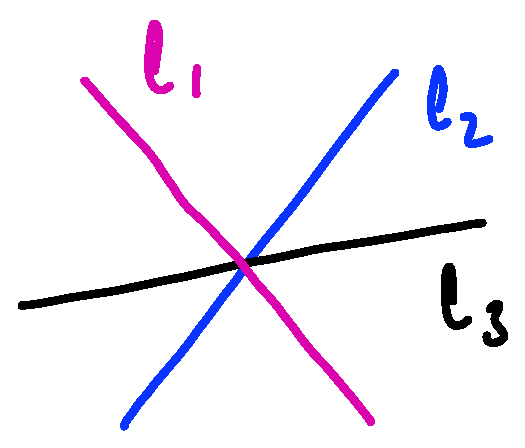
\includegraphics[width=0.35\columnwidth]{indirect-sum-example}
  
    \caption{Пример трёх одномерных подпространств: прямые $l_1, l_2, l_3$, лежащие в одной плоскости. Их сумма не прямая, хотя все попарные пересечения $l_i \hm\cap l_j$, $i \hm{\not=} j$ дают нулевое подпространство.}
    \label{fig:indirect-sum-example}
  \end{figure}
  
  
  \subsection{Пример на пересечение и сумму из аналитической геометрии, где от самой аналитической геометрии по сути лишь ``художественное условие'', а после перехода к координатам природа объектов ``отходит на второй план''}
  \label{sec:example-with-geome-vectors}
  
  Возьмём трёхмерное пространство векторов~---~направленных отрезков.
  И рассмотрим в нём два подпространства: плоскость $\alpha$ ($L_1$) и не параллельную ей плоскость $\beta$ ($L_2$).
  Очевидно, в этом случае плоскости \emph{пересекаются} по прямой, то есть множество векторов, общих и для $\alpha$, и для $\beta$, образует прямую~(\ref{fig:combined-example}).
  Как найти эту прямую?
  
  \begin{figure}[h]
    \centering
  
    \includegraphics[width=0.5\columnwidth]{combined-example}
  
    \caption{Две плоскости $\alpha$ и $\beta$ (двумерные подпространства геометрического пространства векторов) пересекаются по прямой~$l$.}
    \label{fig:combined-example}
  \end{figure}
  
  Пусть в пространстве выбран ортонормированный базис.
  И пусть известно, что вектор нормали плоскости $\alpha$ есть вектор $\bds n_1(0, 1, 0)$, а вектор нормали плоскости $\beta$ есть $\bds n_2(1, 0, 0)$.
  Тогда на плоскости $\alpha$ можно выбрать базис $(\bds a_1, \bds a_2)$ с векторами $\bds a_1(1, 0, 1)$ и $\bds a_2(1, 0, 0)$.
  А на плоскости $\beta$ базисом может быть пара векторов $(\bds b_1, \bds b_2)$, где $\bds b_1(0, 1, 1)$ и $\bds b_2(0, 1, 0)$.
  
  Зная базисы, подпространства можно описать следующим образом:
  \[
    L_1 = \mathcal L(\bds a_1, \bds a_2) = \{t_1 \bds a_1 + t_2 \bds a_2 \mid t_1, t_2 \in \RR\}
  \]
  \[
    L_2 = \mathcal L(\bds b_1, \bds b_2) = \{h_1 \bds b_1 + h_2 \bds b_2 \mid h_1, h_2 \in \RR\}
  \]
  
  Что есть пересечение $L_1 \hm\cap L_2$?
  По определению это:
  \[
    L_1 \cap L_2 = \{\bds v \mid \bds v \in L_1, \bds v \in L_2\}
  \]
  
  При этом условия принадлежности вектора $\bds v$ из пересечения $L_1 \hm\cap L_2$ каждому из подпространств $L_1$ и $L_2$ по отдельности можно представить так ($\alpha_1, \alpha_2, \beta_1, \beta_2 \hm\in \RR$):
  \begin{equation}\label{eq:l1-cap-l2}
    \underbrace{\alpha_1 \bds a_1 + \alpha_2 \bds a_2}_{\bds v \in L_1} = \bds v = \underbrace{\beta_1 \bds b_1 + \beta_2 \bds b_2}_{\bds v \in L_2}
  \end{equation}
  
  Приравняв представления $\bds v$ через базисные из разных подпространств и собрав потом все слагаемые в одной части, получим:
  \[
    \alpha_1 \bds a_1 + \alpha_2 \bds a_2 - \beta_1 \bds b_1 - \beta_2 \bds b_2 = \bds 0
  \]
  
  Иными словами, то, что вектор $\bds v$ лежит в пересечении, равносильно существованию коэффициентов $\alpha_1$, $\alpha_2$, $\beta_1$ и $\beta_2$, при сложении с которыми векторы $\bds a_1$, $\bds a_2$, $-{\bds b_1}$ и $-{\bds b_2}$ дают в сумме ноль.
  Найдя эти коэффициенты, найдём и пересечение.
  (При этом можно заметить, что если система $\{\bds a_1, \bds a_2, \bds b_1, \bds b_2\}$ линейно независима, то только их тривиальная линейная комбинация равна нулю, и потому в пересечении $L_1 \hm\cap L_2$ будет только нулевой вектор.)
  
  Далее можно от работы с векторами (направленными отрезками) перейти к работе с их координатными столбцами:
  \[
    \alpha_1 \begin{pmatrix}
      1\\ 0\\ 1
    \end{pmatrix} + \alpha_2 \begin{pmatrix}
      1\\ 0\\ 0
    \end{pmatrix} - \beta_1 \begin{pmatrix}
      0\\ 1\\ 1
    \end{pmatrix} - \beta_2 \begin{pmatrix}
      0\\ 1\\ 0
    \end{pmatrix} = \begin{pmatrix}
      0\\ 0\\ 0
    \end{pmatrix}
    %%
    \Leftrightarrow \begin{pmatrix}
      1 & 1 &  0 &  0\\
      0 & 0 & -1 & -1\\
      1 & 0 & -1 &  0\\
    \end{pmatrix} \begin{pmatrix}
      \alpha_1\\ \alpha_2\\ \beta_1\\ \beta_2
    \end{pmatrix} = \begin{pmatrix}
      0\\ 0\\ 0
    \end{pmatrix}
  \]

  Упростив матрицу полученной системы, получаем решение:
  \begin{equation}\label{eq:matrix-simplification-in-example}
    \begin{pmatrix}
      1 & 1 &  0 &  0\\
      0 & 0 & -1 & -1\\
      1 & 0 & -1 &  0\\
    \end{pmatrix} \sim \begin{pmatrix}
      1 & 0 & 0 & 1\\
      0 & 1 & 0 & -1\\
      0 & 0 & 1 & 1
    \end{pmatrix}
    %%
    \leftrightarrow \left\{
      \begin{aligned}
        &\alpha_1 = -\beta_2\\
        &\alpha_2 = \beta_2\\
        &\beta_1 = -\beta_2
      \end{aligned}
    \right.
    %%
    \Leftrightarrow
    \begin{pmatrix}
      \alpha_1\\
      \alpha_2\\
      \beta_1\\
      \beta_2
    \end{pmatrix} = t \begin{pmatrix}
      -1\\
      1\\
      -1\\
      1
    \end{pmatrix},\quad t \in \RR
  \end{equation}

  Вернёмся к ``двоякому представлению'' вектора из пересечения подпространств $L_1$ и $L_2$~(\ref{eq:l1-cap-l2}), подставив найденные коэффициенты:
  \[
    L_1 \ni -t \bds a_1 + t \bds a_2 = \bds v = -t \bds b_1 + t \bds b_2 \in L_2
  \]
  \[
    t (\bds a_2 - \bds a_1) = t (\bds b_2 - \bds b_1)
  \]

  Левая и правая части равны, но вектор слева, натянутый на $\bds a_2 \hm- \bds a_1$, лежит в $L_1$, а вектор справа, натянутый на $\bds b_2 \hm- \bds b_1$, лежит в $L_2$.
  Подставляя координаты векторов, можно убедиться, что равенство в самом деле выполняется\footnote{Символ $\leftrightarrow$ в этой формуле, до этого, и далее в конспекте, если ещё встретится, означает ``взаимно однозначное соответствие''. В том смысле, который должен быть понятен из контекста. Например, векторы линейного пространства можно отождествлять с их координатными столбцами в выбранном базисе (в этом случае можно бы было вообще просто ``равно'' $=$ использовать, но хотя бы один раз, ``показательно'', поставим именно ``стрелку'' $\leftrightarrow$).}:
  \[
    \bds a_2 - \bds a_1
    \leftrightarrow \begin{pmatrix}1\\ 0\\ 0\end{pmatrix} - \begin{pmatrix}1\\ 0\\ 1\end{pmatrix}
    = \begin{pmatrix}0\\ 0\\ -1\end{pmatrix}
    = \begin{pmatrix}0\\ 1\\ 0\end{pmatrix} - \begin{pmatrix}0\\ 1\\ 1\end{pmatrix}
    \leftrightarrow \bds b_2 - \bds b_1
  \]
  Таким образом, пересечение, как и предполагалось изначально (из ``геометрических соображений''), получилось одномерным.
  И в качестве базиса в нём можно выбрать, например, $\bds a_2 \hm- \bds a_1$.
  
  \medskip
  
  Как искать сумму $L_1 \hm+ L_2$?
  Можно воспользоваться~(\ref{eq:sum-as-l-basises}): чтобы найти базис в сумме, надо объединить базисы слагаемых $(\bds a_1, \bds a_2, \bds b_1, \bds b_2)$ и убрать ``лишние'' векторы.
  Как понять, какие лишние?
  Можно составить матрицу из координатных столбцов векторов $(\bds a_1, \bds a_2, \bds b_1, \bds b_2)$ и упростить её методом Гаусса: элементарные преобразования строк не меняют линейной зависимости между столбцами, поэтому базисные столбцы в упрощённой матрице будут соответствовать векторам, которые и составляют базис в сумме $L_1 \hm+ L_2$.
  
  Но матрица уже была упрощена ранее~(см.~(\ref{eq:matrix-simplification-in-example}), только в третьем и четвёртом столбцах стояли компоненты векторов $-{\bds b_1}$ и $-{\bds b_2}$):
  \[
    \begin{pmatrix}
      1 & 1 &  0 &  0\\
      0 & 0 & -1 & -1\\
      1 & 0 & -1 &  0\\
    \end{pmatrix} \sim \begin{pmatrix}
      1 & 0 & 0 & 1\\
      0 & 1 & 0 & -1\\
      0 & 0 & 1 & 1
    \end{pmatrix}
  \]
  
  Видно, что первые три столбца~---~базисные.
  Значит, базис суммы~---~это, например, $(\bds a_1, \bds a_2, \bds b_1)$.
  Также видно, что последний столбец в упрощённой матрице раскладывается по базисным следующим образом:
  \[
    \begin{pmatrix}1 \\ -1 \\ 1\end{pmatrix}
    = \begin{pmatrix}1 \\ 0 \\ 0\end{pmatrix} - \begin{pmatrix}0 \\ 1 \\ 0\end{pmatrix} + \begin{pmatrix}0 \\ 0 \\ 1\end{pmatrix}
  \]
  
  Можно убедиться, что точно такая же зависимость есть и между столбцами исходной матрицы:
  \[
    (-{\bds b_2}) = \bds a_1 - \bds a_2 + (-{\bds b_1})
  \]
  
  Глядя на упрощённую матрицу~(\ref{eq:matrix-simplification-in-example}), можно ещё заметить следующее.
  Столбцов в матрице всего $2 \hm+ 2$~---~взяли базисные из $L_1$ и из $L_2$.
  При этом три столбца оказались базисными~---~базис в сумме.
  И один столбец, соответствующий ``свободной'' переменной в системе~---~именно количество параметрических переменных определило размерность пересечения.
  Приведённое наблюдение можно сформулировать в виде формулы:
  \[
    \boxed{\dim(L_1 + L_2) = \dim L_1 + \dim L_2 - \dim(L_1 \cap L_2)}
  \]
  
  
  \section{Задачи}
  
  \subsection{\# 20.23(4)}
  
  Составить систему уравнений, определяющую линейную оболочку системы столбцов:
  \[
    \mathcal L(\bds c_1, \bds c_2) = \{\alpha \bds c_1 + \beta \bds c_2 \mid \alpha, \beta \in \RR\}
  \]
  \[
    \left\{
      \begin{aligned}
        &\bds c_1 = (1, 1, 1, 1)^T\\
        &\bds c_2 = (1, 2, 1, 3)^T
      \end{aligned}
    \right.
  \]
  
  \begin{solution}
    \[
      \begin{pmatrix}
        x_1 \\ x_2 \\ x_3 \\ x_4
      \end{pmatrix} = \alpha \begin{pmatrix}
        1 \\ 1 \\ 1 \\ 1
      \end{pmatrix} + \beta \begin{pmatrix}
        1 \\ 2 \\ 1 \\ 3
      \end{pmatrix}
    \]
    
    Переходим к системе скалярных уравнений (относительно $\alpha$, $\beta$):
    \begin{equation}\label{p-20-23-system}
      \left\{
        \begin{aligned}
          &x_1 = \alpha + \beta\\
          &x_2 = \alpha + 2\beta\\
          &x_3 = \alpha + \beta\\
          &x_4 = \alpha + 3\beta
        \end{aligned}
      \right.
    \end{equation}
    
    Далее, чтобы найти условия на $x_i$ из системы~(\ref{p-20-23-system}), можно взять расширенную матрицу системы, и после упрощения приравнять нулю компоненты в последнем столбце, соответствующие нулевым строкам в основной матрице\footnote{Теорема Кронекера-Капелли.}:
    \[
      \left(
        \begin{matrix}
          \textcolor{pink}{\bds 1} & 1\\
          1 & 2\\
          1 & 1\\
          1 & 3
        \end{matrix} \BigMiddleFour \begin{matrix}
          x_1 \\ x_2 \\ x_3 \\ x_4
        \end{matrix}
      \right)
      \sim \left(
        \begin{matrix}
          1 & 1\\
          0 & \textcolor{pink}{\bds 1}\\
          0 & 0\\
          0 & 2
        \end{matrix} \BigMiddleFour \begin{matrix}
          x_1 \\ x_2 - x_1 \\ x_3 - x_1 \\ x_4 - x_1
        \end{matrix}
      \right)
      \sim \left(
        \begin{matrix}
          1 & 0\\
          0 & 1\\
          0 & 0\\
          0 & 0
        \end{matrix} \BigMiddleFour \begin{matrix}
          2x_1 - x_2 \\ x_2 - x_1 \\ x_3 - x_1 \\ x_4 + x_1 - 2x_2
        \end{matrix}
      \right)
      \Rightarrow \left\{
        \begin{aligned}
          &x_3 - x_1 = 0\\
          &x_4 + x_1 - 2x_2 = 0
        \end{aligned}
      \right.
    \]
  \end{solution}
  
  
  \subsection{\# 21.9}
  
  Найти размерность и базис суммы и пересечения подпространств $L_1$ и $L_2$ пространства многочленов степени не выше третьей:
  \[
    L_1 = \mathcal L(1 + 2t + t^3, 1 + t + t^2, t - t^2 + t^3)
  \]
  \[
    L_2 = \mathcal L(1 + t^2, 1 + 3t + t^3, 3t - t^2 + t^3)
  \]
  
  \begin{solution}
    Множество многочленов степени не выше третьей в самом деле образуют пространство (с ``интуитивными'' операциями сложения многочленов и умножения многочлена на число).
    Так, если есть многочлен $p(t) \hm= a_0 \hm+ a_1 t \hm+ a_2 t^2 \hm+ a_3 t^3$ и многочлен $q(t) \hm= b_0 \hm+ b_1 t \hm+ b_2 t^2 \hm+ b_3 t^3$, то их сумма~---~тоже многочлен степени не выше третьей:
    \[
      (p + q)(t) = p(t) + q(t) = (a_0 + b_0) + (a_1 + b_1) t + (a_2 + b_2) t^2 + (a_3 + b_3) t^3
    \]
    
    Аналогично с умножением многочлена на число: снова получается многочлен степени не выше третьей.
    Операции суммы и умножения на число при этом удовлетворяют всем ``восьми свойствам'' (нулевой многочлен~---~константный ноль).
    Размерность пространства многочленов степени не выше третьей равна $4$, потому что можно выбрать базис из четырёх многочленов
    \[
      e = (1, t, t^2, t^3)
    \]
    
    Начать решение задачи кажется разумным с того, чтобы понять, а какие вообще размерности самих подпространств $L_1$ и $L_2$.
    Можно заметить\footnote{Если не получилось заметить, то можно бы было по-честному искать ``лишние'' многочлены с помощью метода, как, например, при определении базиса в сумме подпространств.}, что
    \[
      (t - t^2 + t^3) = (1 + 2t + t^3) - (1 + t + t^2)
    \]
    и также что
    \[
      (3t - t^2 + t^3) = (1 + 3t + t^3) - (1 + t^2)
    \]
    
    То есть $\dim L_1 \hm= \dim L_2 \hm= 2$.
    Выберем в качестве базисов и в $L_1$, и в $L_2$ по первой паре векторов (многочленов) из трёх, на которые по условию были натянуты каждое из подпространств.
    
    Далее, вместо того, чтобы продолжать работать с многочленами~---~можно перейти к их координатным столбцам в, например, том же ``простом'' базисе~$e$:
    \[
      L_1 = \mathcal L \left\{
        \begin{pmatrix} 1 \\ 2 \\ 0 \\ 1 \end{pmatrix},
        \begin{pmatrix} 1 \\ 1 \\ 1 \\ 0 \end{pmatrix}
      \right\},
      \quad L_2 = \mathcal L \left\{
        \begin{pmatrix} 1 \\ 0 \\ 1 \\ 0 \end{pmatrix},
        \begin{pmatrix} 1 \\ 3 \\ 0 \\ 1 \end{pmatrix}
      \right\}
    \]
    
    А дальше... а дальше всё становится ``очень похоже'' на пример с ``векторами из аналитической геометрии''~(\ref{sec:example-with-geome-vectors})!
    Поэтому... перейдём к следующей задаче.
  \end{solution}
  
  
  \subsection{\# 15.94}
  
  Показать, что любую квадратную матрицу можно разложить в сумму симметрической и кососимметрической.
  Единственно ли такое разложение?
  
  \begin{solution}
    Симметрическая матрица $A$~---~такая что $A \hm= A^T$.
    Кососимметрическая матрица $A$~---~такая что $A \hm= -A^T$.
    
    Можно заметить, что множества симметрических и кососимметрических матриц образуют линейные подпространства в пространстве всех квадратных матриц.
    Покажем это, например, для случая симметрических матриц.
    При умножении на число, очевидно, свойство симметричности сохраняется:
    \[
      (\alpha A)^T = \alpha A^T = \alpha A
    \]
    
    При сложении двух симметрических тоже получим симметрическую:
    \[
      A + B = (a_{ij} + b_{ij})_{ij} = (a_{ji} + b_{ji})_{ij} = (A + B)^T
    \]
    
    Как теперь представить произвольную матрицу в виде суммы симметрической и кососимметрической?..
    
    \bigskip
    
    \emph{Способ 1 (``простой'')}
    
    В предыдущем номере задачника предлагают показать, что матрица $A \hm+ A^T$ симметрическая, а матрица $A \hm- A^T$ кососимметрическая.
    Если это в самом деле так, то, очевидно:
    \[
      A = \frac{1}{2} \bigl((A + A^T) + (A - A^T)\bigr) = \frac{1}{2} (A + A^T) + \frac{1}{2} (A - A^T)
    \]
    То есть разложение произвольной матрицы $A$ в виде суммы двух найдено.
    
    Остаётся в таком случае проверить, что $A \hm- A^T$ в самом деле кососимметрическая (а $A \hm+ A^T$~---~симметрическая):
    \[
      A - A^T = (a_{ij} - a_{ji})_{ij} = -(a_{ji} - a_{ij})_{ij} = -(A - A^T)^T
    \]
    
    Аналогично и с симметричностью матрицы $A \hm+ A^T$.
    
    \bigskip
    
    \emph{Способ 2}
    
    Можно же по-честному записать, что хотим найти:
    \[
      A = X + Y,\quad
      \left\{
        \begin{aligned}
          &X = X^T\\
          &Y = -Y^T
        \end{aligned}
      \right.
    \]
    Представление матрицы $A$ в виде суммы двух и ограничения на матрицы-слагаемые (симметричность одной и кососимметричность другой) можно объединить в одну систему:
    \[
      \left\{
        \begin{aligned}
          &A = X + Y\\
          &X = X^T\\
          &Y = -Y^T
        \end{aligned}
      \right.
    \]
    
    Пусть у матрицы $A$ размер $n \hm\times n$.
    Тогда сейчас в системе $2 \cdot n^2$ неизвестных (количество элементов в матрицах $X$ и $Y$) и $3 \cdot n^2$ уравнений (каждое матричное уравнение равносильно $n^2$ скалярным уравнениям).
    
    Рассмотрим сначала отдельно уравнение $X \hm= X^T$.
    Соответствующая система скалярный уравнений:
    \[
      \left\{
        \begin{aligned}
          &x_{11} = x_{11}\\
          &x_{12} = x_{21}\\
          &\ldots\\
          &x_{21} = x_{12}\\
          &x_{22} = x_{22}\\
          &\ldots
        \end{aligned}
      \right.
    \]
    Таким образом, на самом деле $n$ уравнений вообще ничего не дают (которые для диагональных элементов).
    Другие же позволяют сразу сократить число переменных $x_{ij}$: вместо $n^2$ их теперь (диагональные плюс в одной из половин)
    \[
      n + \frac{n^2 - n}{2} = \frac{n (n + 1)}{2}
    \]
    
    Теперь посмотрим на $Y \hm= -Y^T$:
    \[
      \left\{
        \begin{aligned}
          &y_{11} = -y_{11}\\
          &y_{12} = -y_{21}\\
          &\ldots\\
          &y_{21} = -y_{12}\\
          &y_{22} = -y_{22}\\
          &\ldots
        \end{aligned}
      \right.
    \]
    В этот раз уравнения для диагональных элементов информативны и дают: $y_{11} \hm= \ldots \hm= y_{nn} \hm= 0$.
    Число неизвестных в матрице $Y$ после учёта уравнений $Y \hm= -Y^T$ (половинка без диагонали):
    \[
      \frac{n^2 - n}{2} = \frac{n (n - 1)}{2}
    \]
    
    Остаётся посмотреть на уравнения, соответствующие $A \hm= X \hm+ Y$:
    \[
      \left\{
      \begin{aligned}
        &\left\{
        \begin{aligned}
          &a_{11} = x_{11} + y_{11}\\
          &a_{12} = x_{12} + y_{12}\\
          &\ldots\\
          &a_{1n} = x_{1n} + y_{1n}
        \end{aligned}\right.\\
        &\left\{
        \begin{aligned}
          &a_{21} = x_{21} + y_{21} = x_{12} - y_{12}\\
          &a_{22} = x_{22} + y_{22}\\
          &\ldots\\
          &a_{2n} = x_{2n} + y_{2n}
        \end{aligned}\right.\\
        &\ldots\\
        &\left\{
        \begin{aligned}
          &a_{n1} = x_{n1} + y_{n1}\\
          &a_{n2} = x_{n2} + y_{n2}\\
          &\ldots\\
          &a_{nn} = x_{nn} + y_{nn}
        \end{aligned}\right.
      \end{aligned}
      \right.
    \]
    
    Сначала опять стоит обратить внимание на уравнения с диагональными элементами.
    С их помощью можно сразу найти диагональные элементы матрицы $X$!
    Например
    $
      a_{11} \hm= x_{11} \hm+ y_{11} \hm\Leftrightarrow a_{11} \hm= x_{11}
    $.
    То есть $x_{ii} \hm= a_{ii}$.
    Поэтому общее число неизвестных в матрице $X$ становится равным тоже
    \[
      \frac{n^2 - n}{2} = \frac{n (n - 1)}{2}
    \]
    И общее число неизвестных на данный момент (в обеих матрицах $X$ и $Y$):
    \[
      2 \cdot \frac{n (n - 1)}{2} = n (n - 1)
    \]
    
    И ``неиспользованными'' остались следующие уравнения (с недиагональными элементами матрицы $A$):
    \[
      \left\{
      \begin{aligned}
        &\left\{
        \begin{aligned}
          &a_{12} = x_{12} + y_{12}\\
          &\ldots\\
          &a_{1n} = x_{1n} + y_{1n}
        \end{aligned}\right.\\
        &\left\{
        \begin{aligned}
          &a_{21} = x_{12} - y_{12}\\
          &\ldots\\
          &a_{2n} = x_{2n} + y_{2n}
        \end{aligned}\right.\\
        &\ldots
      \end{aligned}
      \right.
    \]
    И их тоже всего $n (n \hm- 1)$.
    
    Теперь можно заметить, что оставшаяся (до сих пор не очень маленькая) система на самом деле ``распадается'' на много систем из двух уравнений с двумя неизвестными.
    Например, объединяя уравнения с $a_{12}$ и $a_{21}$, получаем:
    \[
      \left\{
        \begin{aligned}
          &a_{12} = x_{12} + y_{12}\\
          &a_{21} = x_{12} - y_{12}
        \end{aligned}
      \right.
    \]
    
    Откуда можно найти $x_{12}$ и $y_{12}$:
    \[
      x_{12} = \frac{a_{12} + a_{21}}{2},\quad y_{12} = \frac{a_{12} - a_{21}}{2}
    \]
    
    И аналогичным образом можно найти все недиагональные элементы в матрицах $X$ и $Y$.
    На самом деле, формулы будут верны и для диагональных элементов.
    Таким образом,
    \[
      x_{ij} = \frac{a_{ij} + a_{ji}}{2},\quad y_{ij} = \frac{a_{ij} - a_{ji}}{2}
    \]
    
    Матрицы $X$ и $Y$ найдены.
    Решение единственное (потому что получено ``по-честному'' как решение системы).
    
    \bigskip
    
    \emph{Способ 3 (``простой Способ 2'')}
    
    Снова ищем матрицы $X$ и $Y$ из соотношения $A \hm= X \hm+ Y$.
    Если же его ещё транспонировать, получим $A^T \hm= X \hm- Y$.
    Имея эти два матричных уравнения, несложно найти матрицы $X$ и $Y$.
    
    В рамках этого способа кажется ещё важным показать отдельно, что решение (пара матриц $X, Y$) единственное.
    Допустим, есть ещё одно разложение матрицы $A$ в виде $X' \hm+ Y'$, где $X'$ симметричная, $Y'$ кососимметричная, и при этом хотя бы $X \hm{\not=} X'$ или $Y \hm{\not= Y'}$.
    Тогда имеем:
    \[
      X + Y = A = X' + Y' \Rightarrow X - X' = Y' - Y
    \]
    
    То есть симметричная равна кососимметричной, при этом хотя бы одна из них ненулевая.
    Противоречие.
  \end{solution}
  
  
  \subsection{\# 21.6(5)}
  
  Найти проекцию вектора $\bds x$ из $\RR^4$ на подпространство $\mathcal P$ параллельно $\mathcal Q$\footnote{То есть предполагается, что $\RR^n = \mathcal P \hm\oplus \mathcal Q$.}.
  Где $\mathcal P$ и $\mathcal Q$~---~линейные оболочки векторов:
  \[
    \mathcal P = \mathcal L \{\bds p_1, \bds p_2\} = \mathcal L \left\{
      \begin{pmatrix}
        1 \\ 1 \\ 1 \\ 1
      \end{pmatrix},
      \begin{pmatrix}
        3 \\ -5 \\ 7 \\ 2
      \end{pmatrix}
    \right\}
    \quad \mathcal Q = \mathcal L \{\bds q_1, \bds q_2\}  = \mathcal L \left\{
      \begin{pmatrix}
        1 \\ 1 \\ 2 \\ 2
      \end{pmatrix},
      \begin{pmatrix}
        1 \\ 1 \\ 1 \\ 3
      \end{pmatrix}
    \right\}
  \]
  а сам вектор $\bds x$ равен
  \[
    \bds x = (1, -7, 5, -2)^T
  \]
  
  \begin{solution}
    Если $\RR^4 \hm= \mathcal P \oplus \mathcal Q$ (что следует из условия задачи), то существует единственное представление вектора $\bds x$ как:
    \[
      \bds x = \underbrace{\alpha \bds p_1 + \beta \bds p_2}_{\pi_{\mathcal P}(\bds x)} + \underbrace{\gamma \bds q_1 + \zeta \bds q_2}_{\pi_{\mathcal Q}(\bds x)}
    \]
    где $\pi_{\mathcal P}(\bds x)$~---~искомая проекция вектора $\bds x$ на $\mathcal P$ параллельно $\mathcal Q$.
    Остаётся составить систему уравнений
    \[
      \begin{pmatrix}
        1 \\ -7 \\ 5 \\ -2
      \end{pmatrix}
      = \alpha \begin{pmatrix}
        1 \\ 1 \\ 1 \\ 1
      \end{pmatrix} + \beta \begin{pmatrix}
        3 \\ -5 \\ 7 \\ 2
      \end{pmatrix} + \gamma \begin{pmatrix}
        1 \\ 1 \\ 2 \\ 2
      \end{pmatrix} + \zeta \begin{pmatrix}
        1 \\ 1 \\ 1 \\ 3
      \end{pmatrix}
    \]
    \[
      \left\{
        \begin{aligned}
          &\alpha + 3\beta + \gamma + \zeta = 1\\
          &\alpha - 5\beta + \gamma + \zeta = -7\\
          &\alpha + 7\beta + 2\gamma + \zeta = 5\\
          &\alpha + 2\beta + 2\gamma + 3\zeta = -2
        \end{aligned}
      \right.
    \]
    
    И решить её методом Гаусса...
    \begin{equation*}
    \begin{split}
      \left(
        \begin{matrix}
          \textcolor{pink}{\bds 1} & 3 & 1 & 1\\
          1 & -5 & 1 & 1\\
          1 & 7 & 2 & 1\\
          1 & 2 & 2 & 3
        \end{matrix}
        \BigMiddleFour
        \begin{matrix}
          1 \\ -7 \\ 5 \\ -2
        \end{matrix}
      \right)
      \sim &\left(
        \begin{matrix}
          1 & 3 & 1 & 1\\
          0 & -8 & 0 & 0\\
          0 & 4 & 1 & 0\\
          0 & -1 & 1 & 2
        \end{matrix}
        \BigMiddleFour
        \begin{matrix}
          1 \\ -8 \\ 4 \\ -3
        \end{matrix}
      \right) \sim \left(
        \begin{matrix}
          1 & 3 & 1 & 1\\
          0 & \textcolor{pink}{\bds 1} & 0 & 0\\
          0 & 4 & 1 & 0\\
          0 & -1 & 1 & 2
        \end{matrix}
        \BigMiddleFour
        \begin{matrix}
          1 \\ 1 \\ 4 \\ -3
        \end{matrix}
      \right) \sim \left(
        \begin{matrix}
          1 & 0 & 1 & 1\\
          0 & 1 & 0 & 0\\
          0 & 0 & \textcolor{pink}{\bds 1} & 0\\
          0 & 0 & 1 & 2
        \end{matrix}
        \BigMiddleFour
        \begin{matrix}
          -2 \\ 1 \\ 0 \\ -2
        \end{matrix}
      \right)\\
      \sim &\left(
        \begin{matrix}
          1 & 0 & 0 & 1\\
          0 & 1 & 0 & 0\\
          0 & 0 & 1 & 0\\
          0 & 0 & 0 & 2
        \end{matrix}
        \BigMiddleFour
        \begin{matrix}
          -2 \\ 1 \\ 0 \\ -2
        \end{matrix}
      \right) \sim \left(
        \begin{matrix}
          1 & 0 & 0 & 1\\
          0 & 1 & 0 & 0\\
          0 & 0 & 1 & 0\\
          0 & 0 & 0 & \textcolor{pink}{\bds 1}
        \end{matrix}
        \BigMiddleFour
        \begin{matrix}
          -2 \\ 1 \\ 0 \\ -1
        \end{matrix}
      \right) \sim \left(
        \begin{matrix}
          1 & 0 & 0 & 0\\
          0 & 1 & 0 & 0\\
          0 & 0 & 1 & 0\\
          0 & 0 & 0 & 1
        \end{matrix}
        \BigMiddleFour
        \begin{matrix}
          -1 \\ 1 \\ 0 \\ -1
        \end{matrix}
      \right)
    \end{split}
    \end{equation*}
    
    Поэтому искомая проекция $\pi_{\mathcal P}(\bds x)$ равна:
    \[
      \pi_{\mathcal P}(\bds x) = -\bds p_1 + \bds p_2
      = -\begin{pmatrix} 1 \\ 1 \\ 1 \\ 1 \end{pmatrix} + \begin{pmatrix} 3 \\ -5 \\ 7 \\ 2\end{pmatrix}
      = \begin{pmatrix} 2 \\ -6 \\ 6 \\ 1 \end{pmatrix}
    \]
  \end{solution}
\end{document}
